\section{Description}


We used various optics to build a Michelson Interferometer (a  complete list will be added at the end of this document.) We had to do several things during the process such as align the beam, mount some delicate optics, and test the end result. 

We mounted the He-Ne laser to the ULM-Tilt base and then placed it on one corner of the breadboard. This was done in such a way as to align the laser beam with the holes on the breadboard. We then had to assemble the silver mirrors onto their mounts. Using slips of paper to stabilize each mirror in its respective mount, we secured them in place. The mounts themselves were then attached to posts and placed in the following locations, shown in the diagram below.

\begin{figure}[ht]
\centering
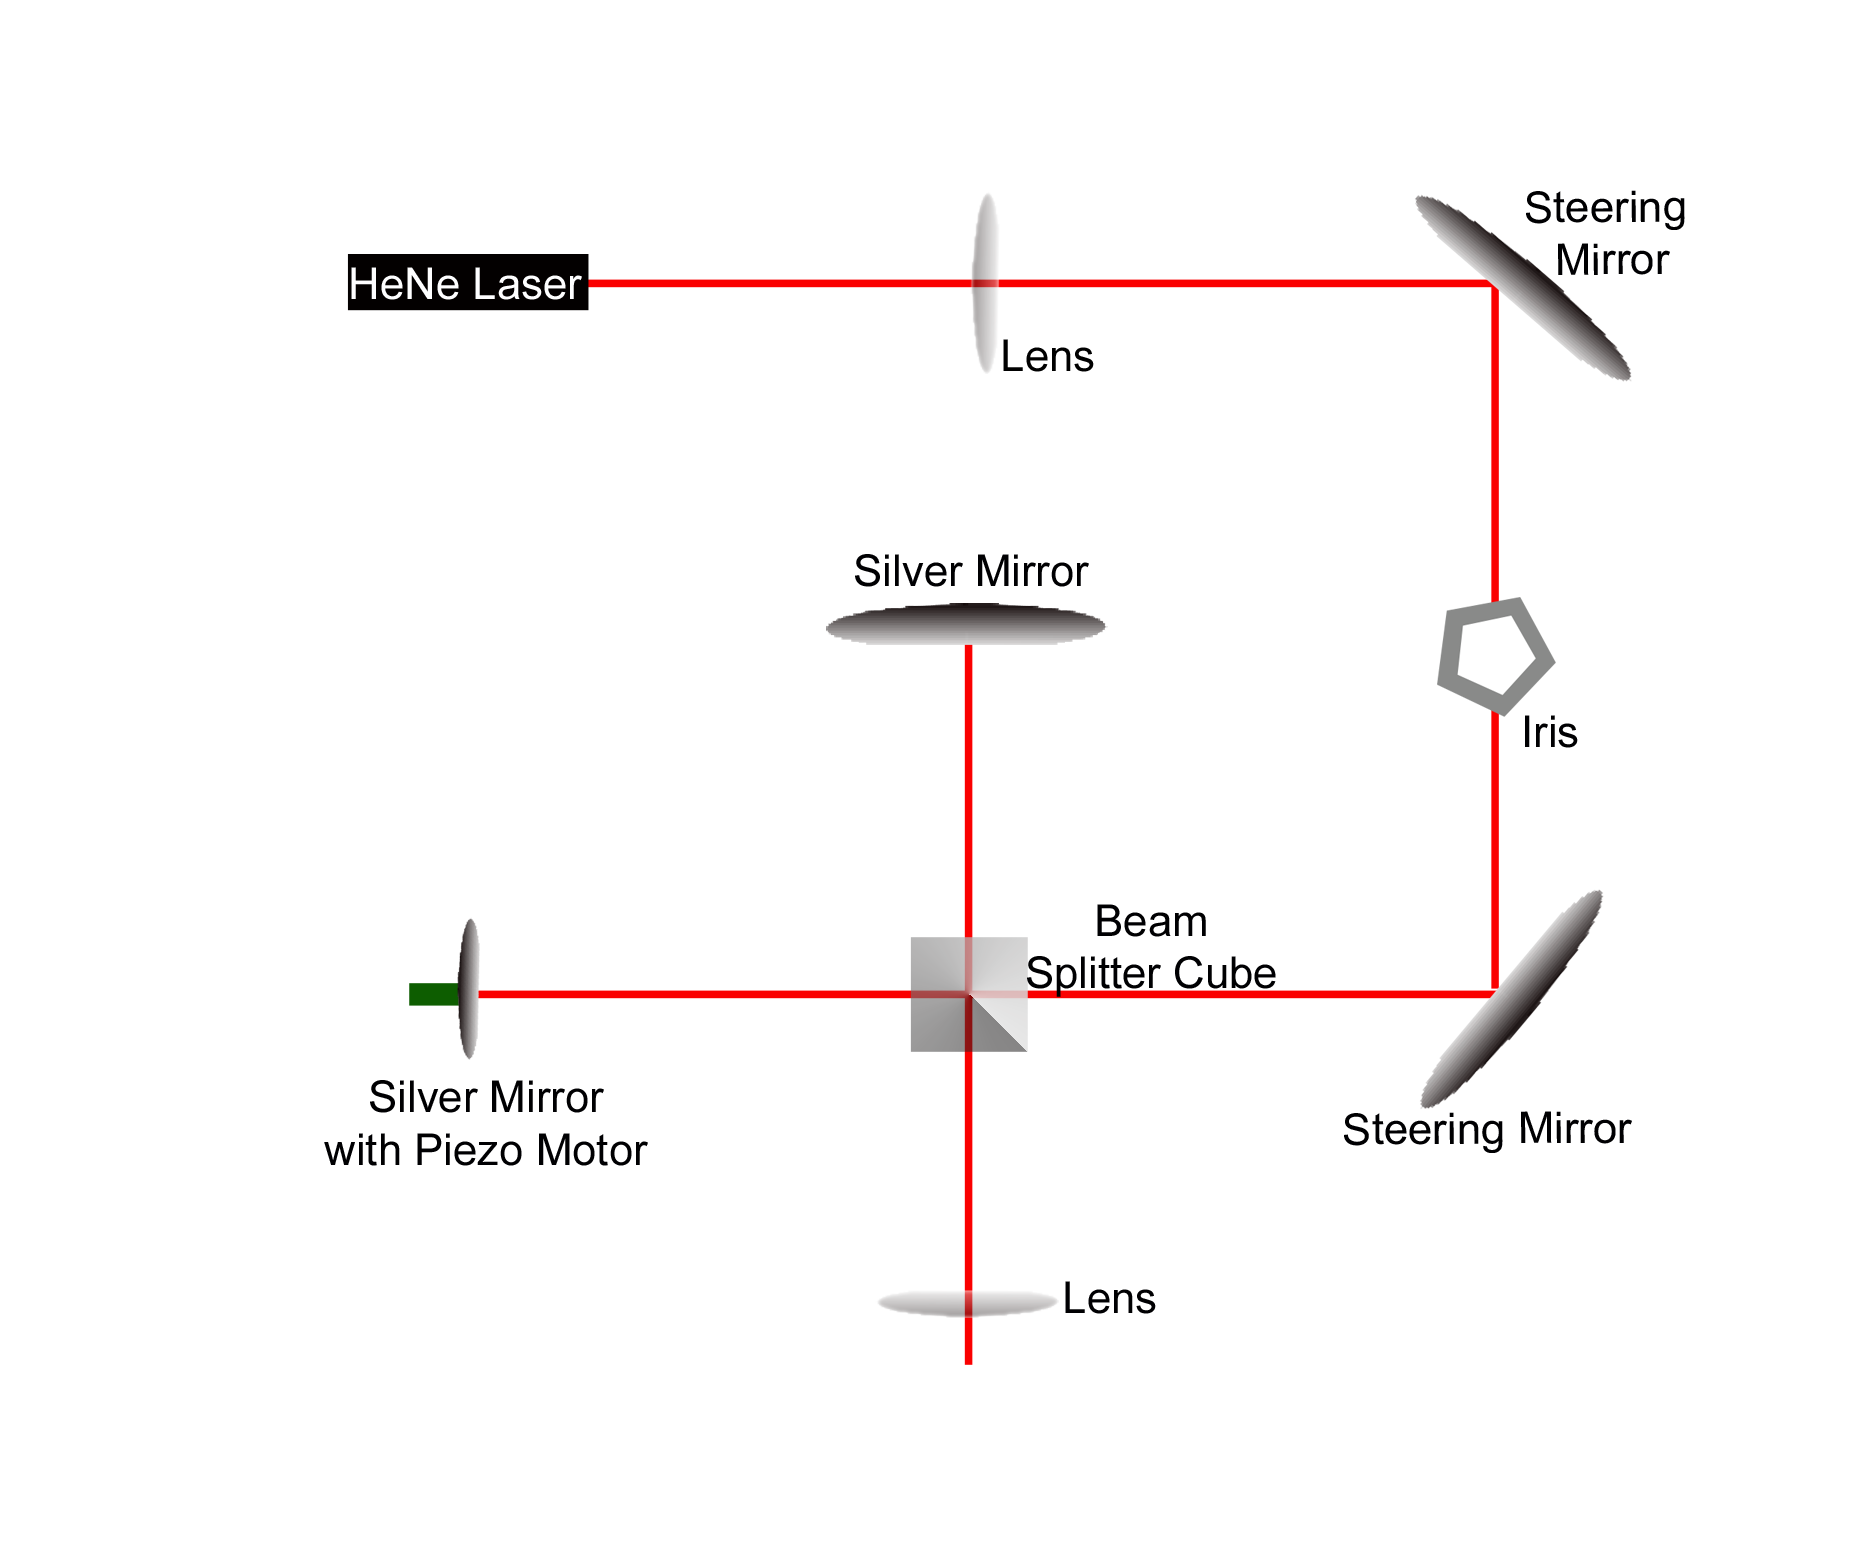
\includegraphics[width=5.5in]{interferometer}
\caption{Interferometer Diagram}
\label{fig:interferometer}
\end{figure}

The next major step we had to overcome was mounting the 0.5 in mirror on the piezo motor, but once in place we simply placed it on a post and set it aside.  Then we carefully mounted the beam splitter cube onto its mount with a small clamping arm. The mounted beam splitter was placed 4.5 inches away from Mirror 1 (the middle mirror in the diagram.) Using the same measurement we placed the Piezo Mirror to the left of the beam splitter.  After setting up this general layout, we turned on the laser to properly align it along the designated path.

The first step in aligning the beam, is to level it out. To do this we used an iris, set at height equal to the mirrors. We then placed the iris between the two steering mirrors to make sure the laser reflected back thru the iris opening. Minor adjustments of the mirrors were required to ensure this.  To obtain a level beam between the second steering mirror, the beam splitter and the piezo mirror the iris has to be moved along it path. First it is placed right in front of the steering mirror and then moved back to the beam splitter to see whether the beam is angled up or down. We once again made adjustments to the mirror until the beam was basically level. After this, the beam traveled from the steering mirror to thru the beam splitter to the Piezo Mirror and back without too much disparity. The beam splitter shoots off a secondary beam to Mirror 3, we just made minor adjustments to try and center this beam on the mirror. 

At this point we could see two splotches on the sheet of white paper that we placed after Lens 2. By making adjustments to Mirror 3, we were able place one splotch on top of the other and get an interference pattern. By looking at this interference pattern we were able to determine if we had correctly aligned the interferometer. An almost perfect or perfect alignment will yield a circular interference pattern, a black dot surrounded by rings or just rings. By pressing on the table (though had the instrument been less sensitive, by changing the arm lengths with a moving mount) we were able to push the interference pattern through several wavelengths at a time. In order to just move through one fringe set, we used the piezo mirror hooked up to a function generator and we replaced Lens 2 with a Photo Diode Detector which was hooked up to an oscilloscope.






%\subsection{Further Beam Alignment}
%\label{sub:further}
%
%    \subsubsection{First Visualization}
%        \begin{enumerate}
%        \item Place a paper or screen vertically after Lens 2.
%        \item Depending on how well aligned your interferometer is, you should
%        see either two distinct beams, or a single beam with dark banding. If
%        you see two beams, use the alignment screws on Mirror 3 and the Piezo
%        Mirror to align these two beams on screen.
%
%            \emph{Alignment Tips}:
%            \begin{itemize}
%            \item If you see purely vertical banding, your misalignment lies
%            only in the horizontal direction.
%            \item Similarly, if you see purely horizontal banding, your
%            misalignment lies only in the vertical direction.
%            \item Diagonal banding is a combination of both vertical and
%            horizontal banding.
%            \item Curved banding is a good sign, as the misalignment is now
%            minimal.  You should seek the center of curvature of the bands.
%            \end{itemize}
%        \end{enumerate} 
%    \subsubsection{Test your interference}
%
%        The interferometer should be sensitive enough to pick up vibrations in
%        the table and breadboard generated by tapping. These would be seen as
%        dark bands moving on the screen.
%    \subsubsection{Achieving Optimum Focus}
%        \begin{enumerate}
%        \item Set the centerline height of Lens 1 to match all other
%        optics.
%        \item Place Lens 1 into the beam path between the He-Ne laser
%        and Mirror 1, and adjust their position to achieve the best focus
%        visible on the screen.
%        \item Mount the post holders to the board and verify that the beam path
%        is still level throughout the entire interferometer. (Refer to
%        Section~\ref{sub:preliminary} Step~\ref{step:leveling} if needed)
%        \end{enumerate}
%
%
%\subsection{Using the Photo Diode}
%\label{sec:photodiode}
%
%    \subsubsection{Introducing the Photo Diode}
%        \begin{enumerate}
%        \item Replace Lens 2 with the Photo Diode and center the beam on the
%        sensor.
%        \item Connect the Photo Diode to CH1 of the oscilloscope using a BNC
%        cable and the Variable Terminator set to the closest match possible to
%        your oscilloscope's impedance.
%        \item Turn on the voltage bias.
%        \item Now fringes can be seen as fluctuations in the signal.
%        \end{enumerate}